%%%%%%%%%%%%%%%%%%%%%%%%%~~~RELATÓRIO DE MNUM TRABALHO 01-2017~~~%%%%%%%%%%%%%%%%%%%%%%%
%%%%%%%%%%%%%%%%%%%%%%%%%%%%%%%~~OBSERVATÓRIO NACIONAL~~%%%%%%%%%%%%%%%%%%%%%%%%%%%%%%%%
%%%%%%%%%%%%%%%%%%%%%%%%%%%%%~~ VICTOR RIBEIRO CARREIRA~~%%%%%%%%%%%%%%%%%%%%%%%%%%%%%%%
%------------------------------------------------------------------------------------------------------------------------------------------%
					             %MODELO DE DOCUMENTO%
%-------------------------------------------------------------------------------------------------------------------------------------------------------%
\documentclass[12pt,a4paper,final]{report}%modelo do documento tipo relatório



%-------------------------------------------------------------------------------------------------------------------------------------------------------%
										   %PACOTES UTILADOS%
%-------------------------------------------------------------------------------------------------------------------------------------------------------%
%\documentclass[border = 60pt]{standalone}
%\usepackage[landscape]{geometry}
%\usepackage{tikz}
%\usetikzlibrary{mindmap}
%\usepackage{metalogo}
%\usepackage{dtklogos}

%\documentclass[border=10pt]{standalone}

%%%%%%%%%%%%%%%%

\usepackage{tikz}
\usetikzlibrary{arrows,calc,positioning}

\tikzstyle{intt}=[draw,text centered,minimum size=6em,text width=5.25cm,text height=0.34cm]
\tikzstyle{intl}=[draw,text centered,minimum size=2em,text width=2.75cm,text height=0.34cm]
\tikzstyle{int}=[draw,minimum size=2.5em,text centered,text width=3.5cm]
\tikzstyle{intg}=[draw,minimum size=3em,text centered,text width=6.cm]
\tikzstyle{sum}=[draw,shape=circle,inner sep=2pt,text centered,node distance=3.5cm]
\tikzstyle{summ}=[drawshape=circle,inner sep=4pt,text centered,node distance=3.cm]
%%%%%%%%%%%%%%%%%%%%%%%%%
\usepackage{smartdiagram}
\usepackage[utf8x]{inputenc}
\usepackage{ucs}
\usepackage{multicol}
\usepackage[comma,authoryear]{natbib}%citação com parentesis e autor ano
\usepackage[english, brazil]{babel}
\usepackage{amsmath}
\usepackage{amsfonts}
\usepackage{amssymb}
\usepackage[colorlinks = true, linkcolor = blue, urlcolor  = blue, citecolor = blue, anchorcolor = blue]{hyperref}
\usepackage{indentfirst}
\usepackage{setspace}
\usepackage{makeidx}
%\usepackage[table]{xcolor}
\usepackage{graphicx}
\usepackage{color}
\usepackage{lipsum} % Required to insert dummy text. To be removed otherwise
\usepackage{epstopdf}%adiciona imagens em formato eps no pdf.
\usepackage{subfigure}%cria ambientes de multifiguras
\usepackage{float}%coloca as figuras exatamente aonde você quer
%\usepackage[monochrome]{xcolor}%imprime o arquivo final em preto e branco
\usepackage[left=2cm,right=2cm,top=2cm,bottom=2cm]{geometry}
\usepackage{lipsum} % Required to insert dummy text. To be removed otherwise
\usepackage{multicol, blindtext, graphicx}%cria figura na página inteira
\usepackage{booktabs} % To thicken table lines
\usepackage{tikz}%pacote para fazer fluxogramas
\usepackage{verbatim}%
\usetikzlibrary{calc,trees,positioning,arrows,chains,shapes.geometric,decorations.pathreplacing,decorations.pathmorphing,shapes,matrix,shapes.symbols}
\author{Victor Ribeiro Carreira}
\title{Projeto de Doutorado 2016}


%--------------------------------------------------------------------------------------------------------------------------------------------------------%
								%INÍCIO DO RELATÓRIO%
%--------------------------------------------------------------------------------------------------------------------------------------------------------%

\begin{document}
\thispagestyle{empty}% retira a numeração da primeira página


\begin{figure}[H]
\centering
\subfigure{
\includegraphics[scale=1.3]{Imagens/logoON.jpg}}
%\subfigure{
\includegraphics[scale=1.5]{Imagens/logoMCT.png}}
\end{figure}

\vspace{1cm}

\begin{center}
\textbf{MODELAGEM NUMÉRICA DE ONDAS SÍSMICAS}
\end{center}

\vspace{3cm}

\begin{center}
\textbf{PROVA:} CÁLCULO DA CONSTANTE DE PROPORCIONALIDADE.
\end{center}

\vspace{2.5cm}

\begin{center}
\textbf{PROFESSOR:} LEANDRO DI BARTOLO
\end{center}

\begin{center}
\textbf{ALUNO:} VICTOR RIBEIRO CARREIRA
\end{center}

\vspace{10cm}

\begin{center}
- 2017 -
\end{center}


%--------------------------------------O relatório---------------------------------------------------

\pagebreak%
\setstretch{1.5}
\section*{Introdução}

Na migração reversa no tempo a representação sísmica de um modelo de subsuperfície pode ser feita com os parâmetros: velocidades das camadas e geometria dos refletores. Neste trabalho a imagem gerada por um refletor é a superposição das imagens geradas por fontes pontuais ao longo das interfaces. 

\section*{Objetivo}

	 
	 Adaptar algoritmo de propagação de ondas acústicas em Fortran (ou um algoritmo equivalente em Fortran ou qualquer outra linguagem) para a migração
	 reversa no tempo pós-empilhamento (zero offset). O programa deverá ser rodado para dado sintético simples (de poucas
	 camadas e com pequeno contraste de impedância) gerado com o conceito do refletor explosivo, o que é parte integrante do trabalho.
	 Assim, as seguintes etapas devem ser realizadas:
	 
	 1) Geração do dados sintético (seção empilhada) a ser migrado e do modelo
	 de velocidades (usado para gerar o dado e na RTM). Sugestão: adotar um modelo de velocidades de 3 camadas, isto é, com 2 refletores, um plano e paralelo com
	 mergulho e outro com curvatura. O programa de modelagem deve ser empregado 	utilizando o modelo de velocidade gerado. A ideia do modelo do refletor explosivo
	 deve ser utilizada no programa de modelagem para a geração da seção.
	 
	 2) Implementação do algoritmo de migração RTM zero offset e aplicar o
	 algoritmo desenvolvido a seção gerada no item anterior. Dica: O algoritmo de modelagem deve ser adaptado, sendo o modelo de velocidades gerado e a seção
	 sísmica os dados de entrada.
	 
	 O trabalho deve ser enviado para leandrodibartolo@gmail.com e deve constar de um: 
	 
	 (a) relatório descrevendo o trabalho, 
	 
	 (b) do modelo de velocidade gerado e o código fonte utilizado para gerá-lo,
	 
	 (c) da seção 	sísmica sintética gerada em conjunto com o código fonte utilizado para gerá-la, 
	 	 
	 (d) da seção migrada com o algoritmo RTM zero Offset, bem como o código fonte utilizado para gerá-la.

\section*{A problemática envolvida}

%Algumas considerações precisam ser feitas para efeito de cálculo. A primeira delas, é que o flúido é considerado um meio isotrópico\footnote{Meio no qual as forças estáticas cisalhantes são nulas.} com viscosidade zero. E a segunda é que a equação da onda acústica é a sua versão linearizada das duas equações básicas citadas no item \textbf{Introdução}.
%
%A onda acústica é definida pelos seguintes termos:
%
%\begin{itemize}
%\item[$p$] é a variação de pressão ($N/m^{2}$=$Pa$)
%\item[$\vec{v}$] é a velocidade da partícula ($m/s$)
%\end{itemize}
%
%A pressão total é indicada pela variável, $p_{t}$, Eq. \ref{ptotal}
%
%\begin{equation}
%p_{t}=p_{0}+p
%\label{ptotal}
%\end{equation}
%
%Onde $p_{0}$ é chamada pressão hidroestática e $p$ representa as mudanças de pressão causada pelo campo de ondas. Desta forma, de maneira similar a desidade total do flúido pode ser definida como na Eq. \ref{denstotal}:
%
%\begin{equation}
%\rho_{t}=\rho_{0}+\rho
%\label{denstotal}
%\end{equation}
%
%A Fig. \ref{fig1} ilustra o problema da superposição.
%
%\begin{figure}[H]
%\centering
%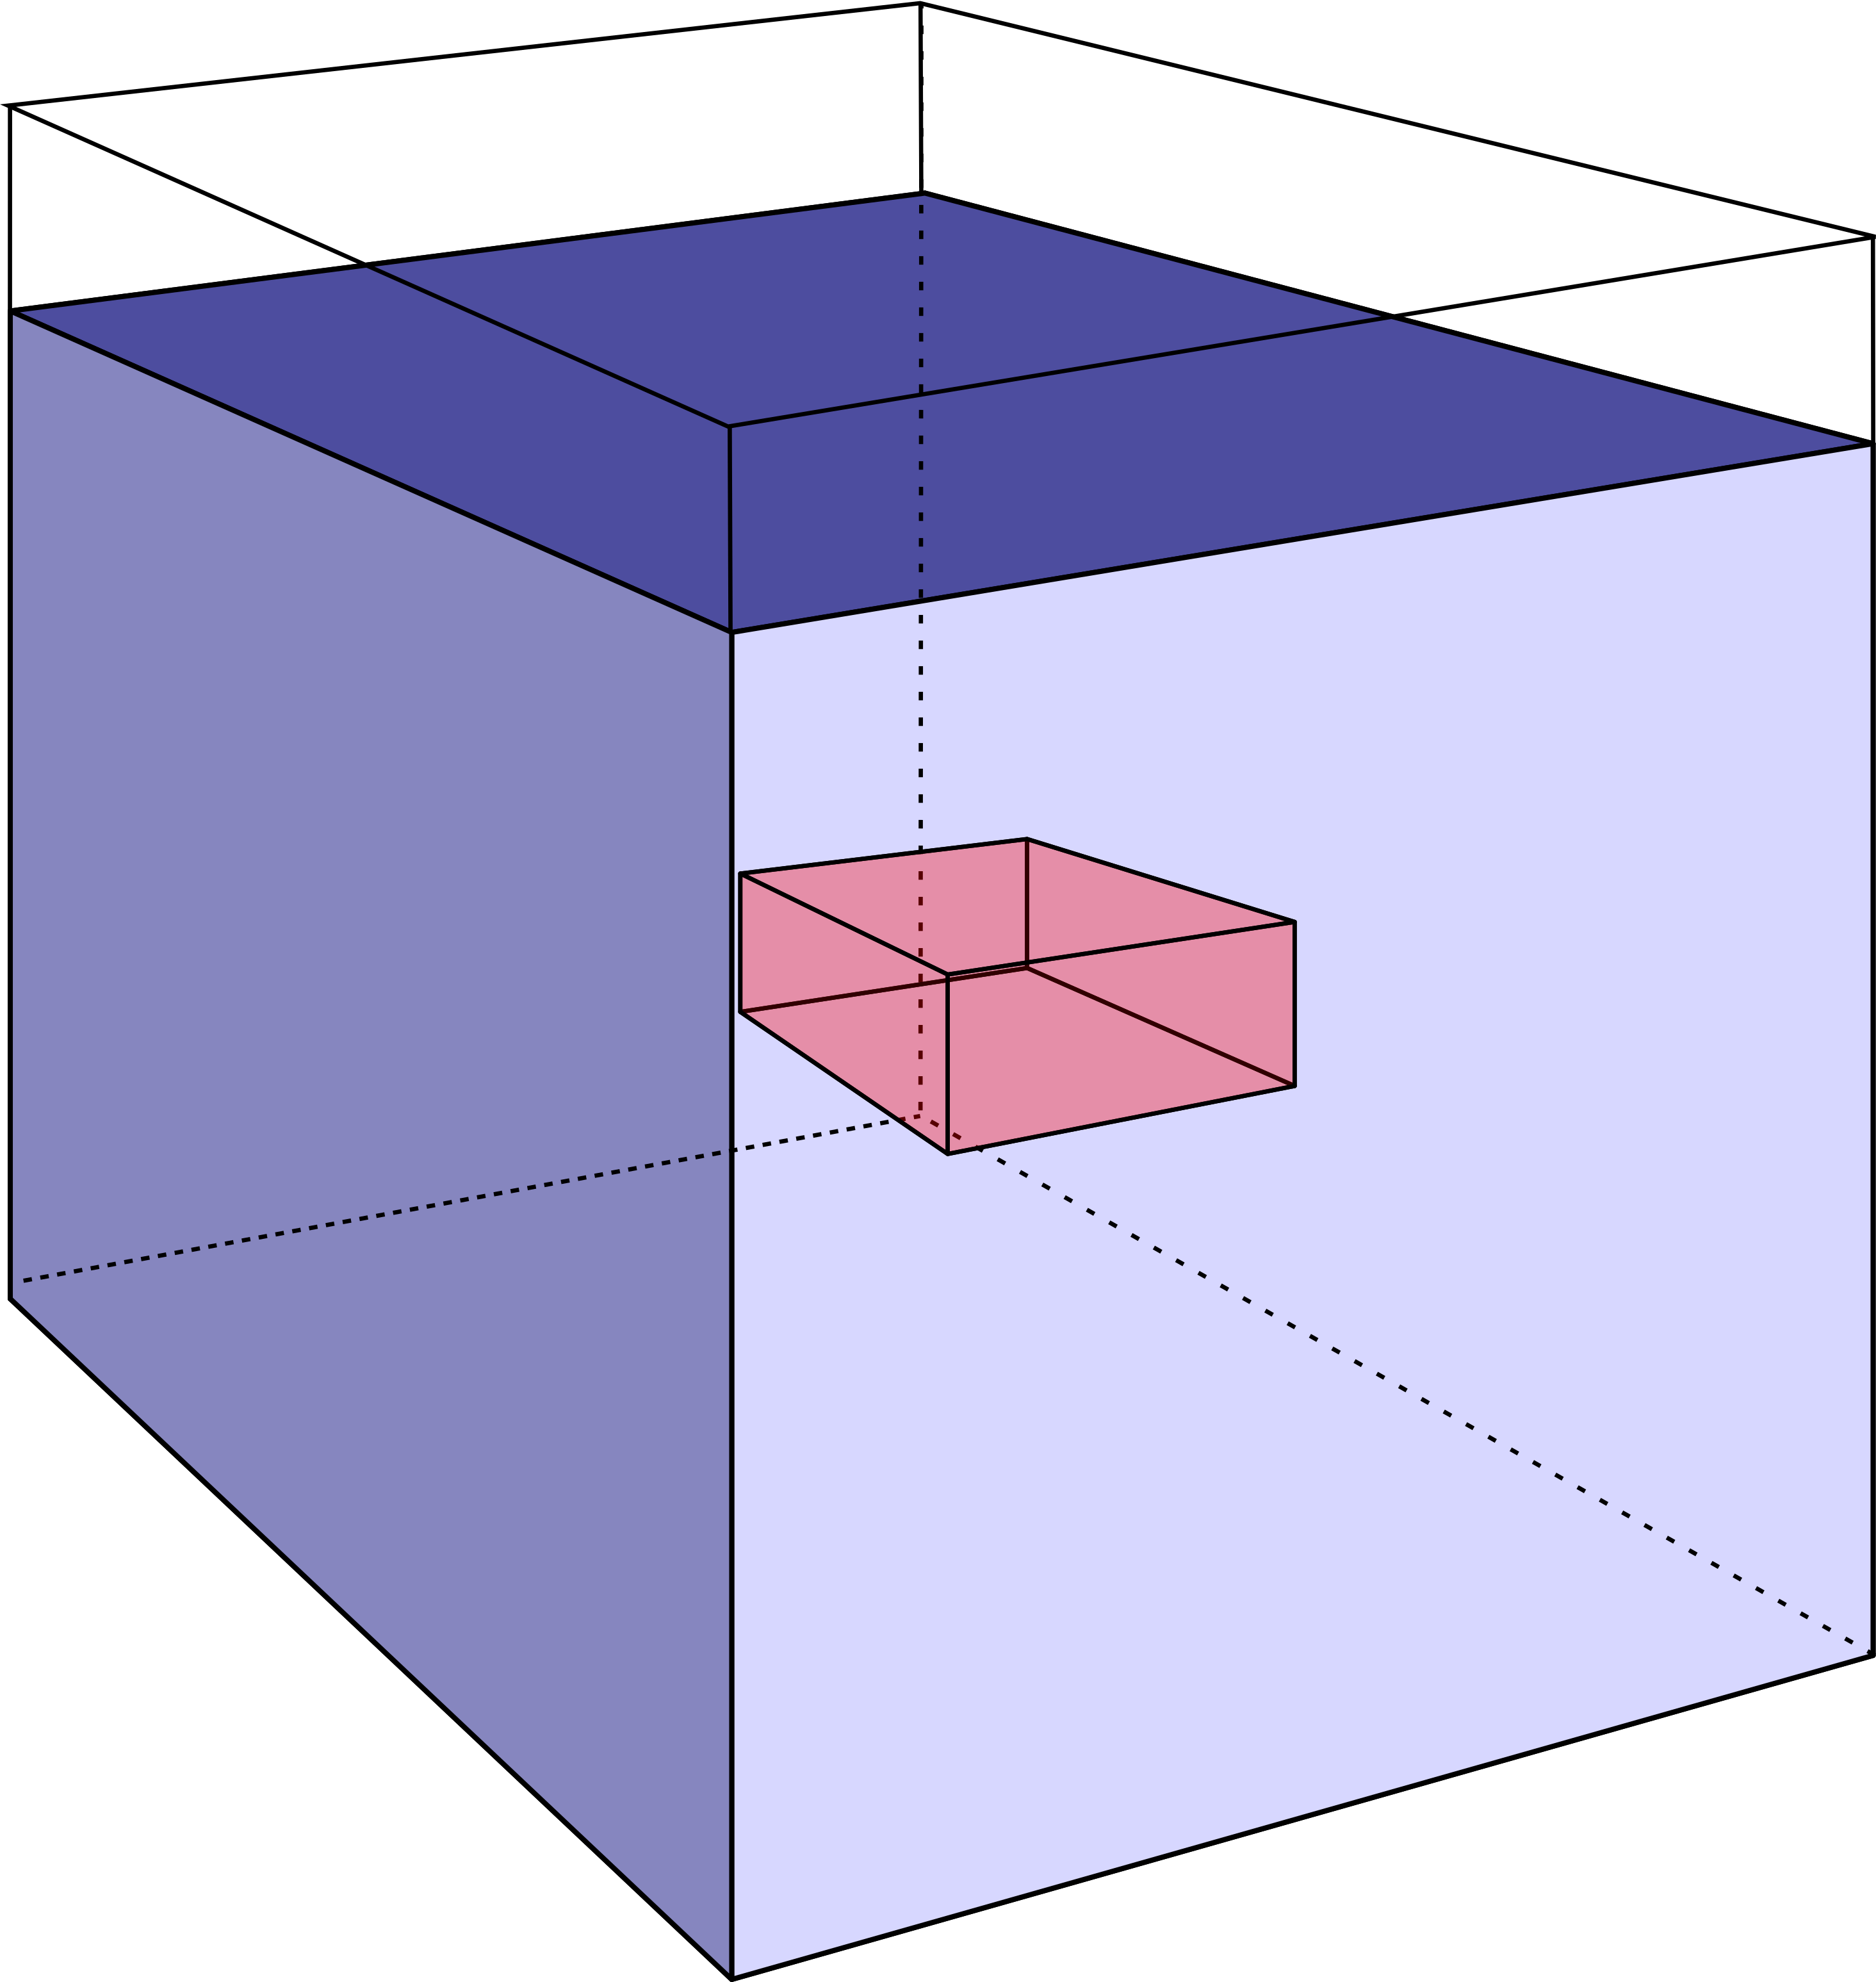
\includegraphics[scale=0.4]{Imagens/CPcubo.png}
%\caption{Ilustração de um cubo (vermelho) imerso em um flúido.}
%\label{fig1}
%\end{figure}


\subsection*{O cálculo}



%-----------------------------------Bibliografia-------------------------------------------------%
%\chapter{Referências}
\bibliographystyle{apalike}
\bibliography{referencias.bib}

\end{document}
